\documentclass[12pt,a4paper]{IEEEconf}
\usepackage[useregional]{datetime2}
\usepackage[pdf]{graphviz}
\usepackage{hyperref}
\usepackage[backend=biber,style=numeric,sorting=none]{biblatex}
\usepackage[utf8]{inputenc}
\usepackage[final]{listings}
\usepackage{color}
\usepackage{amsmath}
\usepackage{xparse}
\usepackage[T1]{fontenc}
\usepackage{enumerate}
\usepackage{CJKutf8}
\usepackage{pifont}
\usepackage{tikz}
\usetikzlibrary{positioning, fit}
\graphicspath{{./images/}}

\definecolor{mygreen}{rgb}{0,0.6,0}
\definecolor{mygray}{rgb}{0.5,0.5,0.5}
\definecolor{mymauve}{rgb}{0.58,0,0.82}
\addbibresource{mergedBib.bib}

% Link conf.
\hypersetup{
    citecolor=blue,
    colorlinks=true,
    linkcolor=blue,
    filecolor=magenta,      
    urlcolor=cyan,
    pdfpagemode=UseNone
}
\urlstyle{same}

% Code conf.
\lstset{ 
  backgroundcolor=\color{white},   % choose the background color; you must add \usepackage{color} or \usepackage{xcolor}; should come as last argument
  basicstyle=\ttfamily\footnotesize,% the size of the fonts that are used for the code
  breakatwhitespace=false,         % sets if automatic breaks should only happen at whitespace
  breaklines=true,                 % sets automatic line breaking
  captionpos=b,                    % sets the caption-position to bottom
  commentstyle=\color{mygreen},    % comment style
  deletekeywords={...},            % if you want to delete keywords from the given language
  escapeinside={\%*}{*)},          % if you want to add LaTeX within your code
  extendedchars=true,              % lets you use non-ASCII characters; for 8-bits encodings only, does not work with UTF-8
  frame=single,	                   % adds a frame around the code
  keepspaces=true,                 % keeps spaces in text, useful for keeping indentation of code (possibly needs columns=flexible)
  keywordstyle=\color{red},        % keyword style
  morekeywords={*,...},            % if you want to add more keywords to the set
  numbers=left,                    % where to put the line-numbers; possible values are (none, left, right)
  numbersep=5pt,                   % how far the line-numbers are from the code
  numberstyle=\tiny\color{mygray}, % the style that is used for the line-numbers
  rulecolor=\color{black},         % if not set, the frame-color may be changed on line-breaks within not-black text (e.g. comments (green here))
  showspaces=false,                % show spaces everywhere adding particular underscores; it overrides 'showstringspaces'
  showstringspaces=false,          % underline spaces within strings only
  showtabs=false,                  % show tabs within strings adding particular underscores
  stepnumber=1,                    % the step between two line-numbers. If it's 1, each line will be numbered
  stringstyle=\color{mymauve},     % string literal style
  tabsize=4,	                     % sets default tabsize to ˋ spaces
  title=\lstname,                  % show the filename of files included with \lstinputlisting; also try caption instead of title
  extendedchars=true,
}

% \font\mytitle=cmr12 at 30pt

\title{{The Container Security in Healthcare Data Exchange System}}
\author{Chih-Hsuan Yang\\
National Sun-Yet-San University, Taiwan \\
Bachelor's degree graduation project \\
Advisor: Chun-I Fan
}

\date{\today}



\begin{document}
% Cover page
\maketitle

%\newpage
%\tableofcontents
%\newpage

% ================ Abstract ================

\section{Abstract}
Recently, many companies use containers to run their microservices, since containers could
make their hardware resources be used efficiently. For example, GCP(Google Cloud Platform),
AWS(Amazon Web Services), and Microsoft Azure are using this technique to separate subscribers'
resources and services. However, if the hacker gets privilege escalation of containers, then
such attacks would influence the host or the other containers.
Therefore, this research would analyze, implement, and protect the container escalation in
healthcare data exchange system.
The container escalation would be inspired in a container and influence the host or the
other containers. The healthcare data exchanging system will take the FHIR(Fast
Healthcare Interoperability Resources)\cite{FHIR_home} to simulate the real world threat and
purpose a secure solution to protect patient's privacy.

% ================ Motivation ================

\section{Motivation}
The Container is a virtualization technique to package applications and dependencies to run in
an isolated environment. Containers are faster to start-up, lighter in memory/storage usage
at run time and easier to deploy than virtual machines. Because the container shares the
kernel with the host OS and other containers, and deploys by a configure file.\\
First, we often used to run a docker container to host our services. For example: assignments,
servers and some services in Information security club at NSYSU(National Sun Yat-sen University).
But there are some threats about container technique. Like "Dirty CoW\cite{Dirty_CoW}"
and "Escape vulnerabilities".\\
"Dirty CoW is a vulnerability in the Linux kernel. It is a local privilege escalation bug
that exploits a race condition in the implementation of the copy-on-write mechanism in the
kernel's memory-management subsystem"\cite{Dirty_CoW_wiki}. It founded by Phil Oester. We
were 16, the first year we had touched the docker container. We tried to use the Dirty CoW
vulnerability to take the root privilege of my Android phone.\\
Escape vulnerability is a subcategory of sandbox security. At first, security researchers often
need sandbox to help they analyze malware, which prevent the malware influence researcher's
host OS. Nowadays, the sandbox not only be used in analyzing, but also used to execute a
normal application for an isolated environment. However if the application could modify the
outside resources without the kernel permission. That loses the purpose of isolation. That
might cause the information leaked or the kernel be hacked.\\
Hence, there is a big problem about: "How to make sure my services isolated and secure?" The
author of this paper is the leader of Information security club. He should maintain all
the services working perfectly. Moreover we are information security club. Therefore,
the security and performance issue is the top-priority requirement.\\
Second, in order to present the container security, we would take the medical system for
example.
The medical system is the most famous part internationally. Including face the COVID-19
in Taiwan, we not have the local COVID-19 case in more than 250 days.\cite{COVID19_CNN}
However, the medical profession needs to renew the exchanging EHR(electronic health records)
system these years. In order to protect the privacy of patients, and producing the high
performance system to exchange the EHR, we need a easy deployment, effective runtime, and
secure system. We have to do this research in this project.

% ================ Related works ================

\section{Related works}
This section will focus on (\RN{1}) \hyperlink{concepts}{concepts} (\RN{2}) \hyperlink{security}{security}, and (\RN{3})
\hyperlink{heigh_performance}{high performance}.

\subsection{Concepts}
\hypertarget{concepts}{}
\subsubsection{Virtual machines and containers}
Different names are used to refer to containers in the literature including OS level
virtualization and lightweight virtualization\cite{Road_Ahead}. However the virtual
machines are providing functionality of a physical computer. The virtual machines
would take a copy of the guest OS, and execute with the virtualization layer on
the host OS. Which difference shows in Figure: \ref*{VM_cont}
\begin{figure}
  \begin{center}
    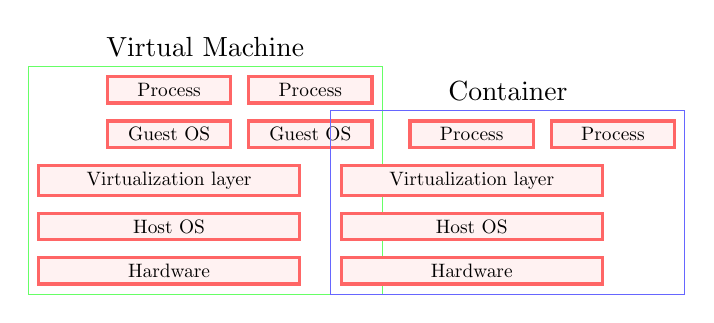
\begin{tikzpicture}[squarednode/.style={align=center, rectangle, draw=red!60,
            fill=red!5, very thick, scale=0.7}]
      % VM
      \node[squarednode] (hardware)[text width=4.5cm]                               {Hardware};
      \node[squarednode] (host) [text width=4.5cm,above=2mm of hardware]            {Host OS};
      \node[squarednode] (virtualization) [text width=4.5cm, above=2mm of host]     {Virtualization layer};
      \node[squarednode] (guest) [text width=2cm, above=2mm of virtualization]      {Guest OS};
      \node[squarednode] (guest1) [text width=2cm, right=2mm of guest]              {Guest OS};
      \node[squarednode] (process) [text width=2cm, above=2mm of guest]             {Process};
      \node[squarednode] (process1) [text width=2cm, above=2mm of guest1]           {Process};
      \node[draw=green!60, fit=(hardware)(process)(process1), label={Virtual Machine}] {};

      % Container
      \node[squarednode] (hardware1) [text width=4.5cm, right = 5mm of hardware]    {Hardware};
      \node[squarednode] (host1) [text width=4.5cm, above=2mm of hardware1]         {Host OS};
      \node[squarednode] (virtualization1) [text width=4.5cm, above=2mm of host1]   {Virtualization layer};
      \node[squarednode] (process2) [text width=2cm, above=2mm of virtualization1]   {Process};
      \node[squarednode] (process3) [text width=2cm, right=2mm of process2]          {Process};
      \node[draw=blue!60, fit=(hardware1)(process2)(process3), label={Container}] {};

    \end{tikzpicture}
    \caption[]{Comparison between containers and virtual machines}
    \label{VM_cont}
  \end{center}
\end{figure}
// FIXME: Align the figure

\subsubsection{FHIR}
The FHIR is a standard for healthcare data exchange. The FHIR standard will be used in
in Taiwan in the near future\cite{MOHW_FHIR}. The FHIR will be used to provide the PHR
(Personal Healthcare Records) in Taiwan. Therefore we choose the most popular standard
"FHIR" for the target.

\subsubsection{Linux kernel features}
There are 4 basic features for the abstract containerization services in Linux environment.
The 4 basic features are: (\RN{1}) namespace, (\RN{2}) cgroups, (\RN{3}) capabilities,
and (\RN{4}) seccomp.

In addition, there are 3 terminologies of the computer science related to container security in
the Linux kernel. Which are (\RN{1}) mmap, (\RN{2}) Copy on write, and (\RN{3}) Race condition.

\paragraph{namespaces}
The Linux kernel provides the namespaces to perform the job of isolation and virtualization
of system resources for a collection of processes\cite{Road_Ahead}.
User namespaces can be nested; that is, each user namespace—except the initial ("root")
namespace—has a parent user namespace, and can have zero or more child user namespaces.
\cite{user_namespaces}
The nested namespace would look like the Figure \ref*{Nested}.
\begin{figure}
  \centering
  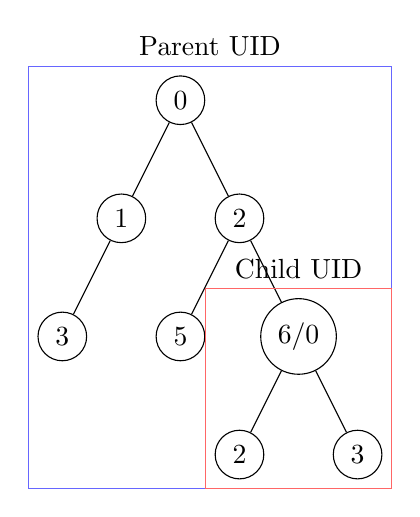
\begin{tikzpicture}[
      roundnode/.style={circle, draw=green!60, fill=green!5, very thick, minimum size=7mm},
      squarednode/.style={rectangle, draw=red!60, fill=red!5, very thick, minimum size=5mm},
    ]
    %Nodes
    \node[circle,draw](z){0}
    child{node[circle,draw]{1} child{node[circle,draw] (p_4){3}} child[missing]}
    child{node[circle,draw]{2} child{node[circle,draw] {5}}
        child{node[circle,draw](n_1){6/0} child{node[circle,draw](n_2){2}} child{node[circle,draw](n_3){3}} } };
    \node[draw=blue!60, fit=(z)(n_2)(n_3)(p_4), label={Parent UID}] {};
    \node[draw=red!60, fit=(n_1)(n_2)(n_3), label={Child UID}] {};

  \end{tikzpicture}
  \caption[]{The nested user namespaces}
  \label{Nested}
\end{figure}

\paragraph{cgroups}
This feature can limit, account for, and isolate the hardware resource usage of a
collection of processes\cite{cgroup_wiki}.
The container could use this feature to set the maximum/minimum usage of hardware
resources, which could guarantee processes' resources using reasonability.

\paragraph{capabilities}
This feature divides the privileges traditionally associated with superuser into
distinct units. For the purpose of performing permission checks, traditional UNIX
implementations distinguish two categories of processes: privileged and unprivileged.
Privileged processes would bypass all kernel permission checks, while unprivileged
processes are subject to full permission checking based on the process's credentials
\cite{capabilities}.

Take ping command for example. The ping needs to generate and receive ICMP packets,
and usually that's done using the "raw sockets" – a feature limited to root only
(CAP\_NET\_RAW). Because it could also be abused to sniff and disrupt other traffic
on the system. And we can set the capability to the file to get accessibility to
execute the file.
Therefore, when we set the CAP\_NET\_RAW capability to the /bin/ping, we could use
the ping command as your user.

\paragraph{seccomp}
The seccomp feature is that only some specified process could call some specified
system calls. We could set a policy of while some file be loaded, and we often use
this system call to enforce the whitelisting or blacklisting policy.

\paragraph{mmap}
This is a system call of mapping files or devices in to memory, which creates a
new mapping in the virtual address space of the caller process. Such that
the process could operate the instance of file in memory directly.
And some libraries are also mapped into the virtual address space to share and handle
the function call. Therefore, the processes could take the same view of libraries in
it's memory space.

\paragraph{Copy on write}
This mechanism purposes of a resource being duplicated but not modified, it is not
necessary to create a new entry. Therefore the kernel can make callers share
the same memory resources. The mmap is a system call could inspire this mechanism
in above paragraph. When some processes request same memory resource, the kernel
supplies the same memory page to callers.

\paragraph{Race condition}
That is processes or threads are racing the same mutable resource. For example:
There is a accessible and mutable shared memory which be initialized as 0. And there
are 2 threads or processes sharing that page. Consider one of the tasks is assigning
the page full of character 'A'. In the meanwhile, the schedular context switches to
the other task, which assigns that page full of 'B'. Then the schedular context switches
again to the first task. There is a problem now. What is the page for the first
task looked like? Obviously, it does not meet the expectation for the first task.
This is race condition.

\subsection{Security}
\hypertarget{security}{}
\subsubsection{Study of the Dirty Copy On Write}
This paper\cite{Study_Dirty_Cow} show the race condition, and the mechanism of
"copy on write". "Copy on write" is "a resource-management technique used in
computer programming to efficiently implement a "duplicate" or "copy" operation
on modifiable resources." \cite{CoW_wiki} It often be inspire when fork() or mmap().

\subsubsection{Dirty CoW demo code}
Let's analyze the proof of concept(PoC) of dirty CoW.(Oester, 2016)\cite{Dirty_CoW}
The key of inspiring this vulnerability is the mmaped memory space, which is mapped with
the PROT\_READ flag. The PROT\_READ flag declares the page is read only.
\lstinputlisting[language=C, linerange={87-89, 101-101}, firstnumber=87]{src/dirtyc0w.c}

It creates 2 threads, which would have a race condition of the mmaped memory space,
\hyperlink{madvise}{madviseThread} and \hyperlink{procself}{procselfmemThread}.

\hypertarget{threads_main}{threads in main}
\lstinputlisting[language=C, linerange={106-107}, firstnumber=106]{src/dirtyc0w.c}

In one thread, call a system call "madvise", would make the user thread gain the root
privilege to operate the protected page temporary. And the flag MADV\_DONTNEED would
tell the kernel: "Do not Expected access it in the near future.\cite{Madvise}" Moreover,
this flag might not lead to immediate freeing of pages in the range. The kernel is free
to delay free the pages until an appropriate moment.\cite{Madvise}

\hypertarget{madvise}{madviseThread}
\lstinputlisting[language=C, linerange={33-39,45-48}, firstnumber=33]{src/dirtyc0w.c}

In another thread, open its memory resource file. This file is a special file, which allow
the process reads its memory by itself.\\
Than, we move the printer of file descriptor of the memory resource file to the mmaped
space. And try to write it. But the mmaped space is a read only space. We expected the
kernel would create a copy of the this space and write the copy\cite{root_exploit}.\\
\hypertarget{procself}{procselfmemThread}
\lstinputlisting[language=C, linerange={50-53,61-63,67-71}, firstnumber=50]{src/dirtyc0w.c}

But there is a problem! There is an another thread is racing this page with root privilege.
If the schedular context switches the madviseThread to procselfmemThread, while the
adviseThread is calling the "madvise" system call. It would cause the procselfmemThread
gain the root privilege from madviseThread to control the mmaped file.

\subsubsection{Container Security: Issues, Challenges, and the Road Ahead}
This paper\cite{Road_Ahead} has derived 4 generalized container security issues:
(\RN{1}) protecting a container from applications inside it, (\RN{2}) inter-container
protection, (\RN{3}) protecting the host from containers, and (\RN{4}) protecting containers
from a malicious or semi-honest host.\cite{Road_Ahead}

The (\RN{1}), (\RN{3}), and (\RN{3}) issue could implement the protection by the software
based solutions.

For the (\RN{1}) protecting a container from applications, this paper recommends that
we could use the different capabilities and the LSM(Linux secure module). Take
CVE-2017-5123\cite{CVE-2017-5123} for example. The vulnerability here is the third argument of
waitpid() system call didn't ensure that the user specified pointer points to user space
and not kernel space. Since unprivileged users shouldn’t be able to write arbitrarily
to kernel memory.

The solution of CVE-2017-5123 without update the Linux kernel is insert a
LSM to the kernel, which monitor the runtime behaviors of system call. If any process
use the waitpid() with a pointer point to kernel as the third argument, the LSM should block
the operation and raise a signal to user.

For the (\RN{2}) inter-container protection, this paper recommends that we could use the
LSM, namespaces, and cgroups to limit the container. Take CVE-2016-8655\cite{CVE-2016-8655}
for example. This vulnerability is a bug in net/packet/af\_packet.c. We often use the
CAP\_NET\_RAW namespace in container to make unprivileged user could sue some privileged
net-util commands. The bug is there exist a race condition probability to race the unauthorized
data inside packet\_set\_ring() and packet\_setsockopt()\cite{CVE-2016-8655-lwn}.
// FIXME: Explain the code here.

For the (\RN{3}) protecting the host from containers issue.
Take the Dirty CoW vulnerability for example, which is an exploitation from the Linux kernel,
the vulnerability could change the victim container to a privileged container. Therefore, we should
protect the host form the container, which belongs to type (\RN{3}) threat in this paper.

\subsection{High performance}
\hypertarget{heigh_performance}{}
This section will study some IO performance and caching issues. Because the medical
data exchange system demands stringent specification of the response time.
The IO is the most often causing the bottleneck in the low latency required system.
In order to support a high performance system, we can design a module to control
the throughput intelligently, and use the cache friendly architecture to minimal the
latency.

\subsubsection{PINE: Optimizing Performance Isolation in Container Environments}
This paper\cite{Optimizing} introduce a high throughput and low latency module to control
the IO streams. Which implement a module to accord a calculated optimization parameters,
and check if the process throughput is satisfied or the 99.9\% throughput is satisfied.

That is if the throughput reached the bottleneck, then the model would extend the
bandwidth by the cgroup. The latency evaluation is more difficult than throughput
evaluation. This paper\cite{Optimizing} used the statistical data to calculated the
99.9\% of latency is it in the margin of error in 3 standard deviation, if not the
module will raise the priority of the IO queue.

\subsubsection{The epoll vs. io\_uring performance comparison}
// FIXME: Introduce the epoll and the io\_uring.
// FIXME: Mode the introduction to the concepts subsection
// FIXME: Use the [report](https://hackmd.io/@shanvia/B1Ds1vlAD) as reference

% ================ Methods ================

\section{Methods}
This project would use the MapReduce model. As shown in Figure \ref*{Fig:model}.

\begin{figure}
  \centering
  \digraph[scale=0.7]{methFlow}{
  Study[margin="0"]
  Merge[margin="0"]
  "Container\noexpand\n Security"[margin="0"]
  "FHIR\noexpand\nSystem"[margin="0"]

  Study -> "Container\noexpand\n Security"-> Merge
  Study -> "FHIR\noexpand\nSystem" -> Merge
  rankdir=LR
  }
  \caption[]{The mapReduce model in this project}
  \label{Fig:model}
\end{figure}

\subsection{Study}
\subsubsection{Study CVEs and related mechanisms}
The Linux kernel is a monolithic kernel, which is over 28 million lines of codes now(2020). There
are many mechanisms to solve the real life situations. Study those CVEs' related mechanism in the
kernel, might have more chance to find new vulnerabilities.

This project will study several container vulnerabilities for example: CVE-2016-8655
\cite{CVE-2016-8655}, CVE-2016-9962\cite{CVE-2016-9962}, and CVE-2020-14386\cite{CVE-2020-14386}.

And study some kernel exploit techniques\cite{Kernel_exploitation}, because the container shares
the kernel. If I could exploit the kernel in the suffering container, it might have more chance
to influence the other containers or host.

\subsubsection{Study FHIR and related standards}
This project will implement the FHIR\cite{FHIR_home} data exchange system to demonstrate the container
security risk. Hence, we should study FHIR standard, JSON format(RFC7159), XML format(RFC4825), and
RESTful APIs.

\subsubsection{Efficient IO with io\_uring}\cite{Efficient_IO_uring}
This is a new asynchronous I/O API in Linux kernel 5.7. POSIX has aio\_read() and aio\_write() to
satisfy asynchronous IO, however the implementation of those is most often lackluster and performance
is poor. We will study and implement the new asynchronous I/O API: io\_uring in this project to
optimize performance of the FHIR data exchange system.

\subsection{Container Security}
\subsubsection{Implement a simple container}
The Linux kernel supply some system calls to clone a process(also in thread) in their own namespace
and group. We could implement a simple container by ourself, so that we can make a list of
vulnerabilities may happen.
% \begin{lstlisting}
\UseRawInputEncoding\lstinputlisting[language={}]{src/lc_out.txt}
% \end{lstlisting}

\subsubsection{List secure details of the simple container}
In my rough opinion, there are 5 types of container security risks, (\RN{1}) Host OS risks, (\RN{2})
Orchestration system risks, (\RN{3}) Container runtime risks, (\RN{4}) Registry risks, (\RN{5})
Images risks. In this stage we should research the details of those risk, and purpose some solutions.

\paragraph{Host OS risks}
\begin{itemize}
  \item Improper user permission
  \item Kernel vulnerabilities
\end{itemize}

\paragraph{Orchestration system risks}
\begin{itemize}
  \item Unbounded domain access
  \item Weak credentials
  \item Mismanaged inter-container network traffic
  \item Mixed of workload sensitivity levels
\end{itemize}

\paragraph{Container runtime risks}
\begin{itemize}
  \item Runtime software vulnerabilities
  \item Unbounded network access from containers
  \item Insecure container runtime configurations
\end{itemize}

\paragraph{Registry risks}
\begin{itemize}
  \item Insecure connections to registries
  \item Old images in registries
\end{itemize}

\paragraph{Images risks}
\begin{itemize}
  \item Image vulnerabilities
  \item Embedded malware or secrets
\end{itemize}

\subsubsection{Aim a vulnerability and implement the PoC}
After listing the risks. This project would find a vulnerability of privilege escalation in
the container and affect with other containers.

\subsubsection{Implement the patch and pull request}
Being a security researcher, we cannot just only exploit the software, but also give patches to
the maintainer. Make the container technique more secure.

\subsection{FHIR system}
\subsubsection{Front-end}
This project would designed a user friendly interface. Make it easy to get data for the
patient and patient's family. And make the exchange of patient's data between different medical
center confidential, integral, and available.

The interface would be designed as a website. Which make every user could access in different platform.

\subsubsection{Back-end}
This project would use the container technique at the back-end. Would isolate different services in
different container. We would also design a access controller for variadic requests, and
design a high performance kernel module to speed up the IO and caching.

\paragraph{Access controller}
The access controller would be implemented as a kernel module. Because malicious user has fewer
probability to break the Linux kernel, if this module have no bugs.
The access controller would use the the whitelisting method to enforce the accessibility policy.
It would reserve the essential system calls in the container, and discard all unused system calls.

\paragraph{High performance server}
This project would implement a kernel module for the high performance server. Which could hook the IO
system calls from the web server. The module would replace the normal IO calls to asynchronous IO,
which could enhance the concurrency performance to provide high throughput.

Moreover, this project would design an efficient algorithm to predict and cache the container's
application data. To reduce the latency, while backend server requiring data.

\subsection{Merge}
The last step is combining the FHIR system and container security. This project would demonstrate
an escalation of normal container(ie. Docker) to steal patients' information form web server.
However, our container can detect and prevent malicious user escaping the container of web server.

In addition, the performance issue is also the key point in this project. We would provide a
high performance FHIR system for the real life requirement. Therefore, we would also improve the
IO performance at the final stage in this project.

% ================ Expected Outcome ================

\section{Expected Outcome}
This project will implement a high performance FHIR medical data exchange system to demonstrate
the container escalation. We want to deploy FHIR system in containers. The container technique
cloud isolate the environments between different container. Apart from, it is faster to start-up,
lighter in memory/storage usage at run time and easier to deploy than virtual machines.

Therefore, this project have 2 parts: FHIR and container security.
\paragraph{Container security}
We would implement a vulnerability PoC, patch, and demonstration for container escalation.
Hope this research could make the container technique become more secure, and provide the medical
data exchange system more reliable.
\paragraph{FHIR system}
We would implement the medical data exchange system with the FHIR standard. The implementation
considers the most two important issue: security issue and performance issue. Hope this project
could be the medical data exchange system model role of implementation in Taiwan.

\printbibheading[heading=bibnumbered]
\printbibliography\newrefcontext

\section{Academic Advisor}
\begin{itemize}
  \item Give advises of security issues.
  \item Give advises of the front-end of user interface.
  \item Introduce the vision of medical data exchanging system.
  \item Organize this research to a complete structure.
  \item Extend to a formal paper, and publish.
\end{itemize}

\end{document}
